\documentclass[aspectratio=169]{beamer}

\usepackage{graphicx}
\usepackage{subcaption}
\usepackage{bm}

\title{TRC 2019 Project 2 WP 2 Meeting 4}
\author{Eve, Nidish, Paw}

\begin{document}
\maketitle{}

\begin{frame}[allowframebreaks]
  \frametitle{Benchmark 0 (SDOF Linear Harmonic Oscillator)}
  \framesubtitle{Comparison of frequency responses around resonance}
  \begin{itemize}
  \item Linear system simulated for different amplitudes used to train
    PNLSS model (with non-linear order fixed to 3)
  \item The linear part of identified model is compared with  the
    original model using the analytical transfer function
  \item The identified model is also investigated to gain insight into
    issues related to over-fitting
  \item \alert{Matches are perfect}
  \end{itemize}
  \begin{figure}
    \centering
    \begin{subfigure}{0.5\linewidth}
      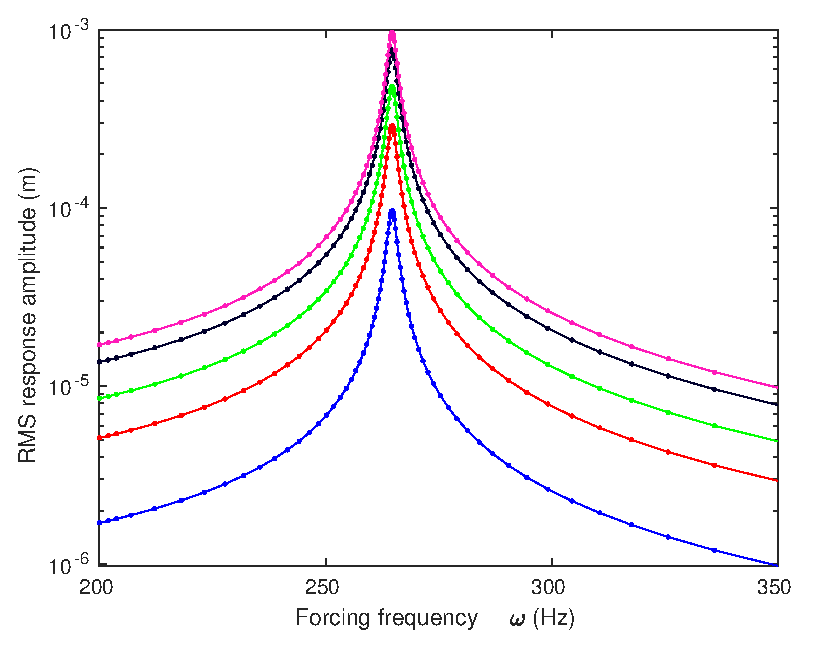
\includegraphics[width=\linewidth]{{../../../benchmark0/fig/pnlsstf_A0.01_Amp_F4096}.eps}
    \end{subfigure}%
    \begin{subfigure}{0.5\linewidth}
      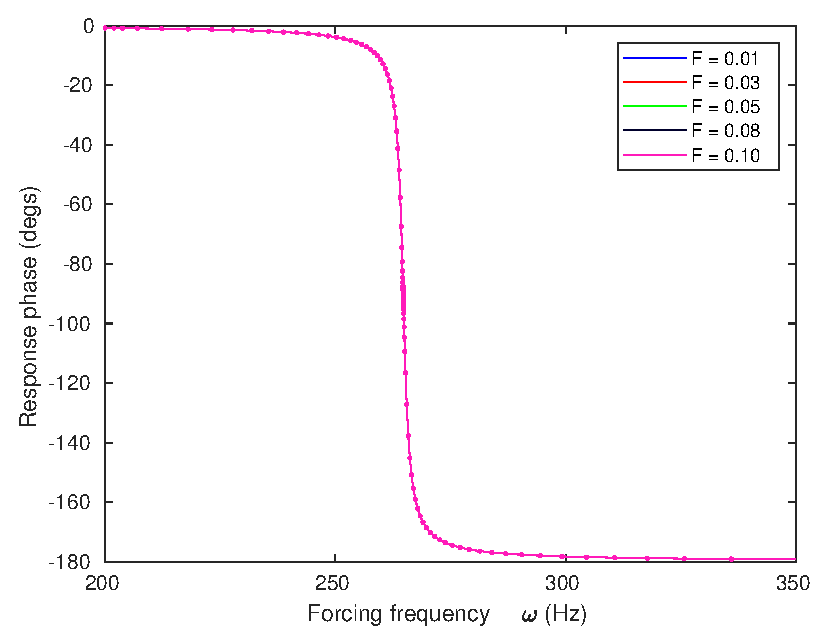
\includegraphics[width=\linewidth]{{../../../benchmark0/fig/pnlsstf_A0.01_Phase_F4096}.eps}
    \end{subfigure}    
    \caption{Comparison of analytical FRFs of linear parts (cont. from
    HB; dotted from identified model). Model from data trained at 0.01N
    rms multisine (150Hz, 400Hz). No amplitude dependence observed (as
    expected)}
\end{figure}

\begin{figure}
  \centering
  \begin{subfigure}{0.5\linewidth}
    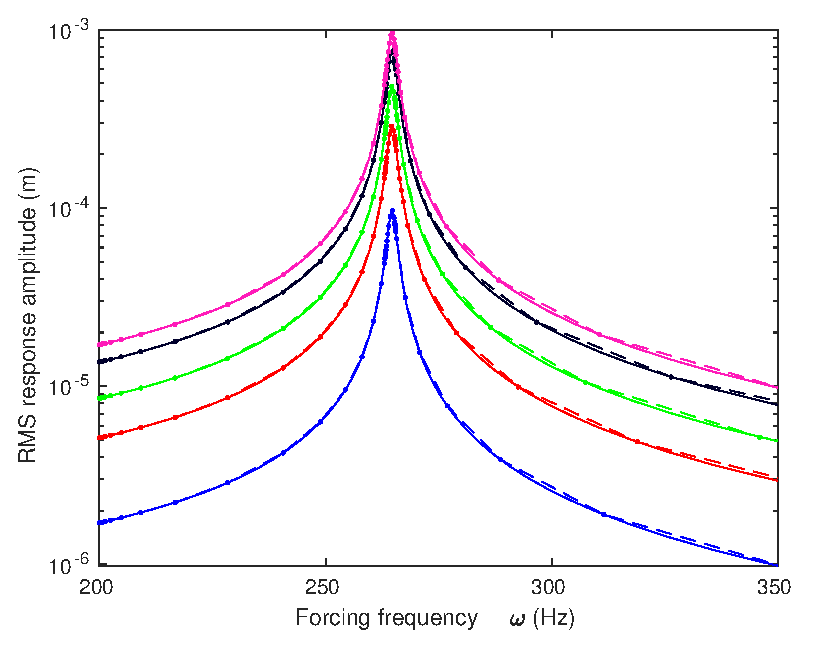
\includegraphics[width=\linewidth]{{../../../benchmark0/fig/pnlssfrf_A0.01_Amp_F4096}.eps}
    \caption{$||u||_2$ = 0.01N}
  \end{subfigure}%
  \begin{subfigure}{0.5\linewidth}
    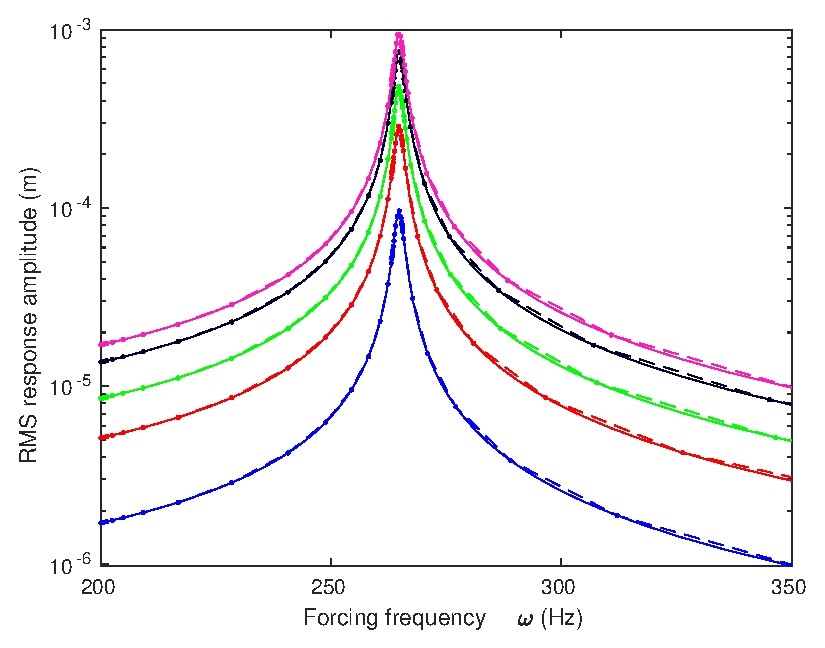
\includegraphics[width=\linewidth]{{../../../benchmark0/fig/pnlssfrf_A0.25_Amp_F4096}.eps}
    \caption{$||u||_2$ = 0.25N}
  \end{subfigure}%  
  \caption{Comparison of simulated FRFs.}
\end{figure}
\end{frame}

\begin{frame}[allowframebreaks]
  \frametitle{Benchmark 1 (SDOF Nonlinear Beam (Duffing oscillator))}
  \framesubtitle{Overview and setup}
  \begin{itemize}
  \item There was a serious scaling issue we debugged a couple of days
    back, which showed us that the amplitudes we were using were
    unrealistically huge
  \item This is fixed now and we have results that are more expectable
  \item We also wanted to compare if both the models estimate the
    stability regimes identically so we just added corresponding
    expressions to the post-processing functions for nlvib
  \end{itemize}
  \textbf{Stability exponents for continuous time HB (Hill's method)}
  \begin{itemize}
  \item This is obtained by solving the quadratic eigenvalue problem,
    \begin{equation}
      \label{eq:1}
      \mathbf{\tilde{J_{NL}}} + \mathbf{\tilde{C}} \lambda +
      \mathbf{\tilde{M}} \lambda^2 = 0.
    \end{equation}
  \item $\mathbf{\tilde{J_{NL}}}$ is the non-linear frequency-domain
    Jacobian; $\mathbf{\tilde{C}}$ \& $\mathbf{\tilde{M}}$ are
    $(eye(2N_h+1) \otimes \mathbf{C})$ \& $(eye(2N_h+1) \otimes
    \mathbf{M})$ respectively
  \item The first $N_d$ exponents closes to the origin are retained.
  \item A solution is stable if $\angle\lambda>90^\circ-1^\circ$
  \end{itemize}
  \textbf{Stability exponents for discrete time HB}
  \begin{itemize}
  \item Starting from the same idea as Hill's method, the perturbed
    solution is taken as
    \begin{equation}
      X_n = X^*_n + s_ne^{\lambda t_n}
    \end{equation}
  \item Subtituting this into the EOM,
    \begin{align}
      X_{n+1} =& \mathbf{A}X_n + \mathbf{B} u_n + \mathbf{E}
                g(X_n)\nonumber\\
      \implies\qquad X^*_{n+1} + =& \mathbf{A}X^*_n + \mathbf{B} u_n + \mathbf{E}
                         g(X^*_n)\nonumber\\
      s_{n+1}e^{\lambda (t_n+\Delta t)}\quad & + \left[ \mathbf{A} +
                                                   \frac{\partial}{\partial
                                                   X}[\mathbf{E}g(X)]\biggr\rvert_{X^*_n}
                                                   \right]s_n
                                               e^{\lambda t_n}
    \end{align}
  \item Applying force balance and using Fourier Ansatz,
  \end{itemize}
  {\small
    \begin{align}
      \begin{bmatrix}1& cos(i\omega t_n)& sin(i\omega
        t_n)\end{bmatrix}\biggl( \begin{bmatrix} \bm{1} & \bm{0} &
        \bm{0}\\\bm{0} & \bm{cos(i\omega\Delta t)} &
        \bm{sin(i\omega\Delta t)}\\ \bm{0} & -\bm{sin(i\omega\Delta
          t)} & \bm{cos(i\omega\Delta
          t)} \end{bmatrix}e^{\lambda\Delta t} -\nonumber\\
      \begin{bmatrix}\bm{A_{nl}}&&\bm{0} \\& \bm{A_{nl}}\\ \bm{0}&&
        \bm{A_{nl}} \end{bmatrix} \biggr) \begin{Bmatrix}S_{a^0}\\ 
        S_{a^i}\\ S_{b^i}\end{Bmatrix} = \begin{Bmatrix} 0 \end{Bmatrix} 
    \end{align}}
  \begin{itemize}
  \item The exponents $\lambda$ are obtained as $log(<eigs>)\times
    fs$.
  \item Once again, only the first $d$ $\lambda$'s are chosen which
    are closest to the origin and interpreted identically to Hill's
    exponents.
  \end{itemize}
\end{frame}

\begin{frame}[allowframebreaks]
  \frametitle{Benchmark 1 (SDOF Nonlinear Beam (Duffing oscillator))}
  \framesubtitle{Looking at the signals \& responses}
  \begin{figure}
    \centering
    \begin{subfigure}{0.33\linewidth}
      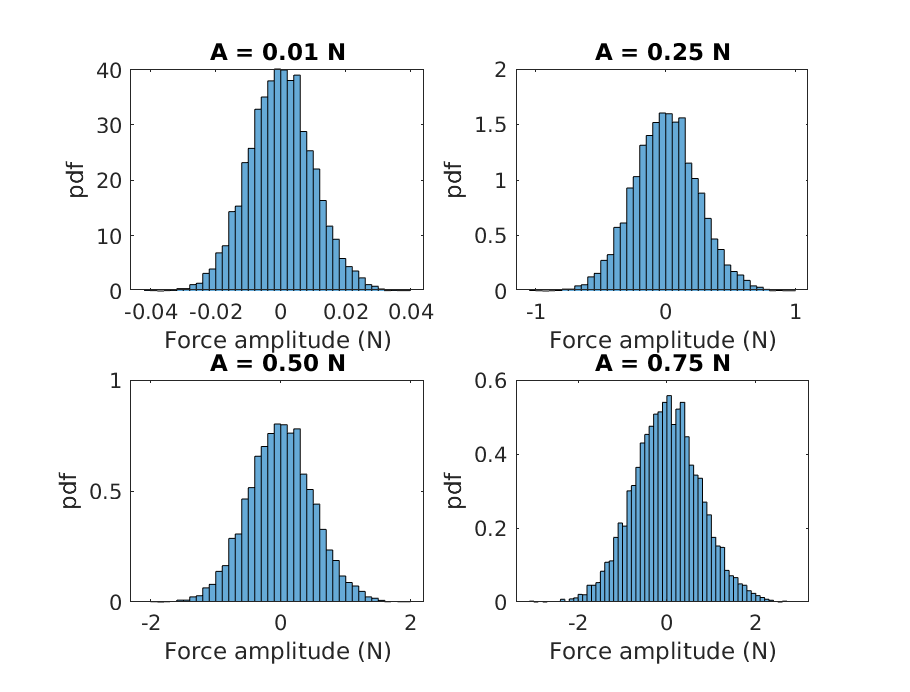
\includegraphics[width=\linewidth]{../../../benchmark1/fig/Excitation_Hists}
      \caption{Excitation}
    \end{subfigure}%
    \begin{subfigure}{0.33\linewidth}
      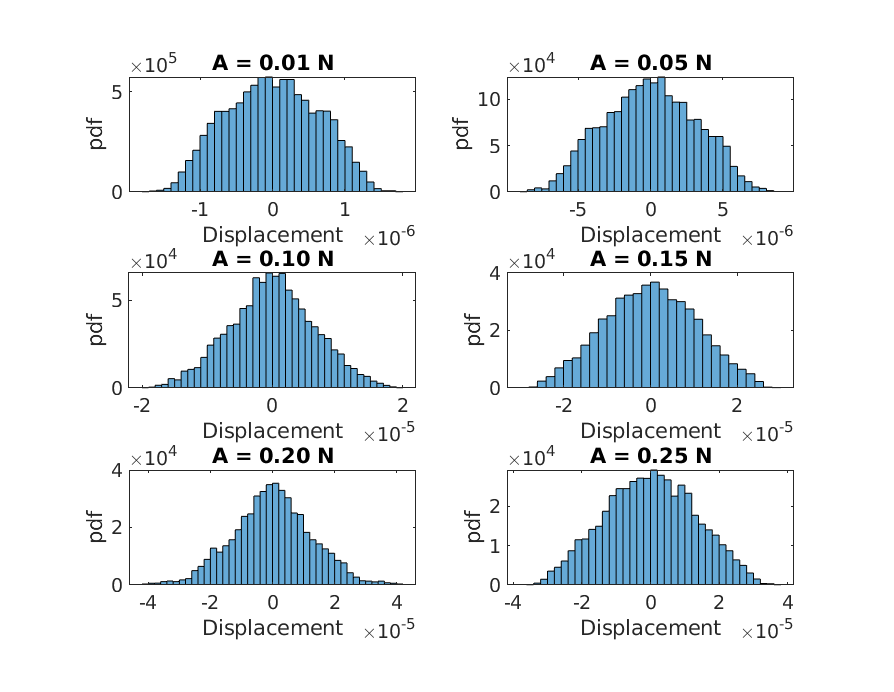
\includegraphics[width=\linewidth]{../../../benchmark1/fig/Response_Hists}
      \caption{Response}
    \end{subfigure}%
    \begin{subfigure}{0.33\linewidth}
      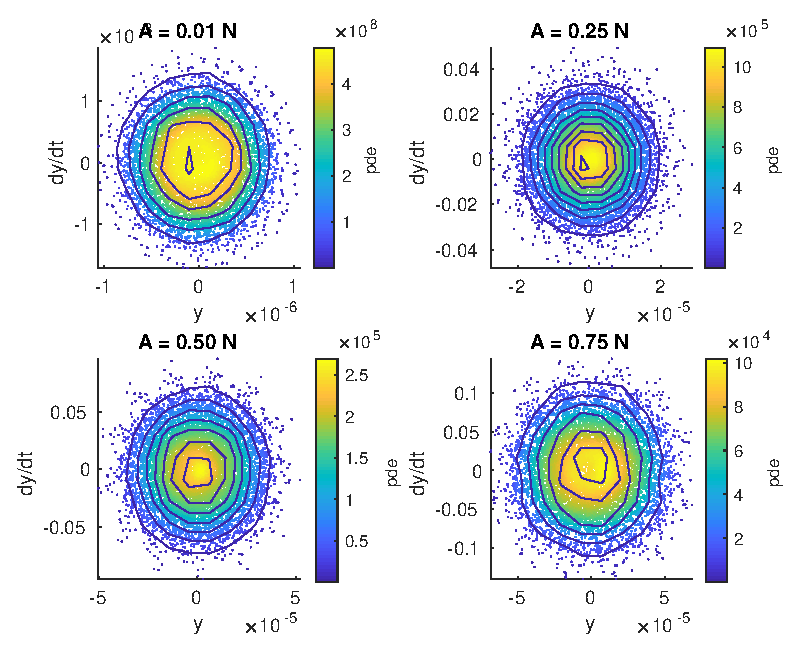
\includegraphics[width=\linewidth]{../../../benchmark1/fig/MS_stateplanekde}
      \caption{State-plane Response}
    \end{subfigure}%    
  \end{figure}
  \begin{itemize}
  \item In the following we plot the responses of the continuous time
    model with stable-continuous lines and unstable-dashed lines
  \item And, the responses of the discrete time model with
    stable-dotted lines and unstable-crossed lines
  \end{itemize}
\end{frame}

\begin{frame}[allowframebreaks]
  \frametitle{Benchmark 1 (SDOF Nonlinear Beam (Duffing oscillator))}
  \framesubtitle{Comparison of frequency responses around resonance}
  \begin{figure}
    \centering
    \begin{subfigure}[t]{0.3\linewidth}
      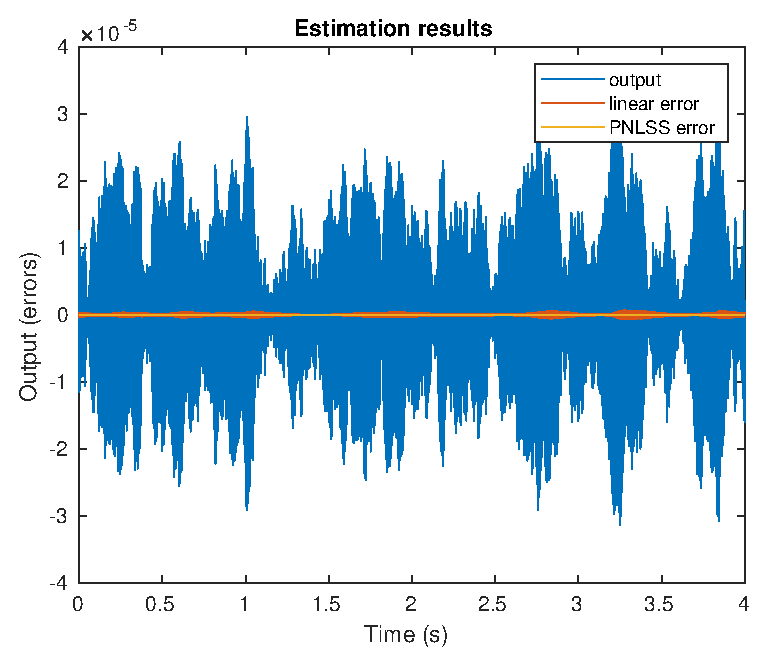
\includegraphics[width=\linewidth]{{../../../benchmark1/fig/TDOMESTRESS_PNLSS_A0.01_F4096}.eps}
      \caption{$u_{rms} = 0.01N$}
    \end{subfigure}%
    \begin{subfigure}[t]{0.3\linewidth}
      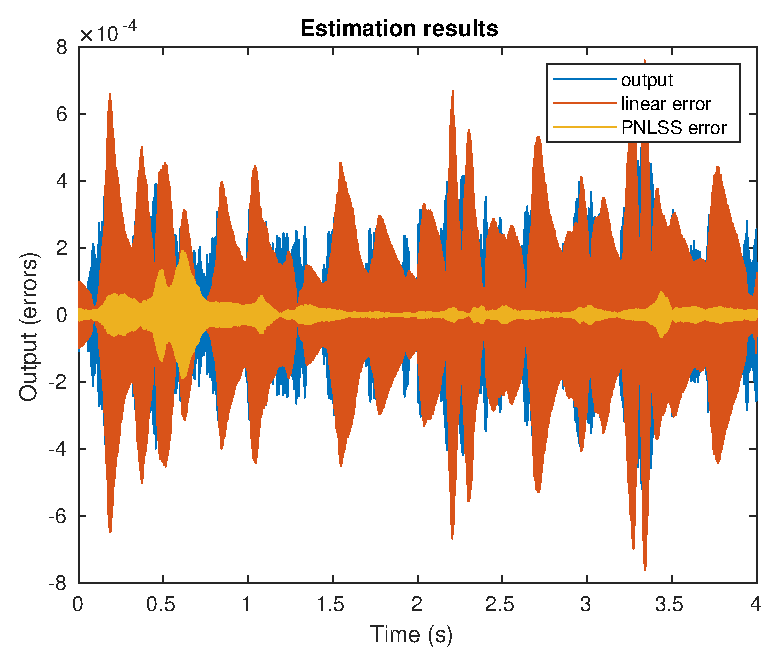
\includegraphics[width=\linewidth]{{../../../benchmark1/fig/TDOMESTRESS_PNLSS_A0.15_F4096}.eps}
      \caption{$u_{rms} = 0.15N$}
    \end{subfigure}%
    \begin{subfigure}[t]{0.3\linewidth}
      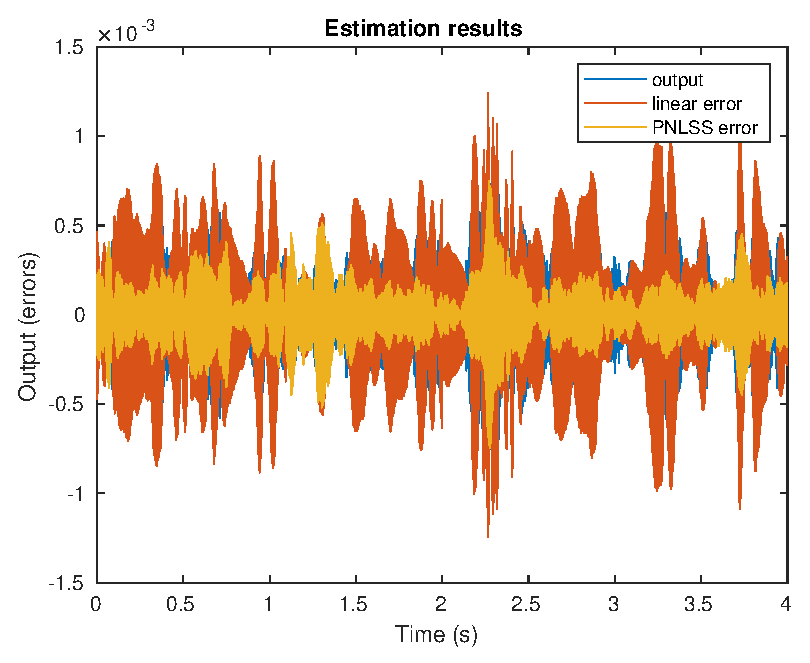
\includegraphics[width=\linewidth]{{../../../benchmark1/fig/TDOMESTRESS_PNLSS_A0.25_F4096}.eps}
      \caption{$u_{rms} = 0.25N$ (non-periodic)}
    \end{subfigure}%
    \caption{Time-domain residues ($n_x=[3]$)}
  \end{figure}
  
  \begin{figure}
    \centering
    \begin{subfigure}[t]{0.25\linewidth}
      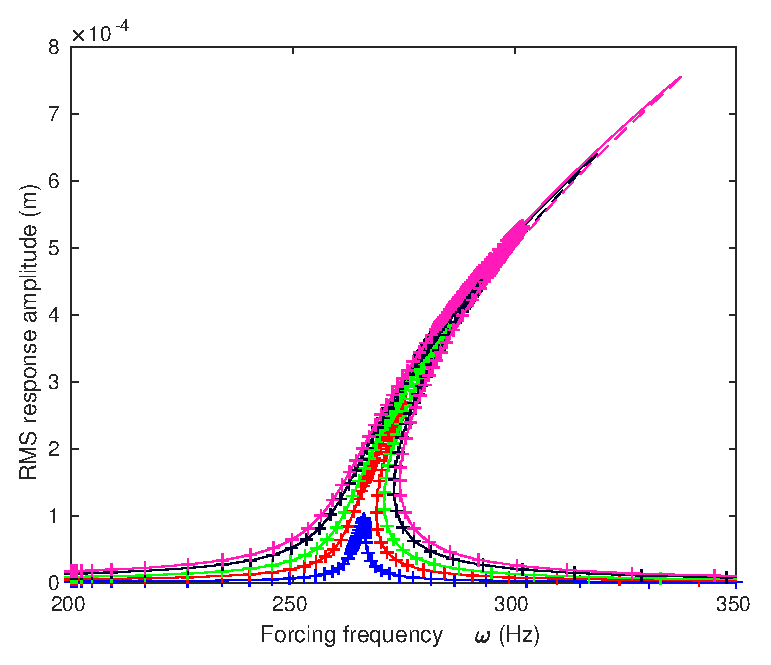
\includegraphics[width=\linewidth]{{../../../benchmark1/fig/pnlssfrf_A0.01_Amp_nx3}.eps}\\
      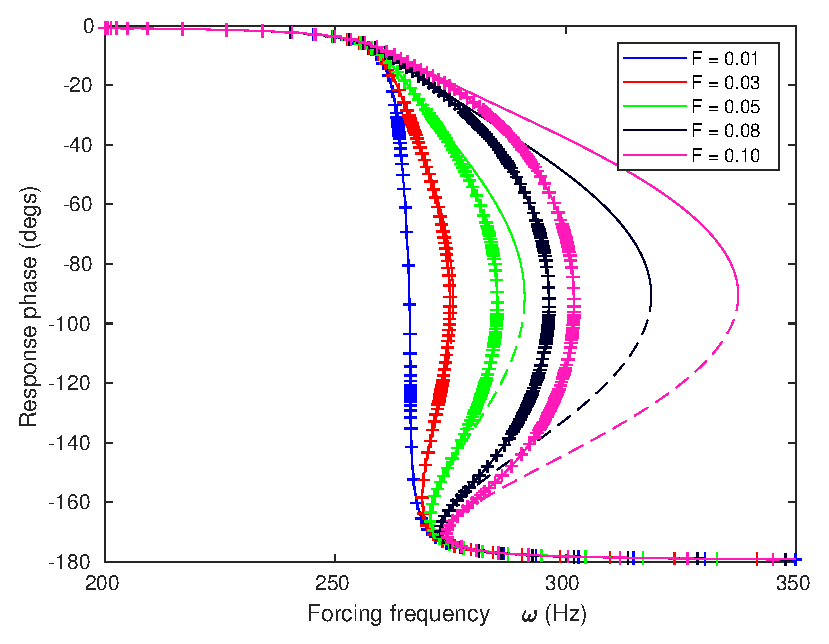
\includegraphics[width=\linewidth]{{../../../benchmark1/fig/pnlssfrf_A0.01_Phase_nx3}.eps}
      \caption{$u_{rms} = 0.01N$}
    \end{subfigure}%
    \begin{subfigure}[t]{0.25\linewidth}
      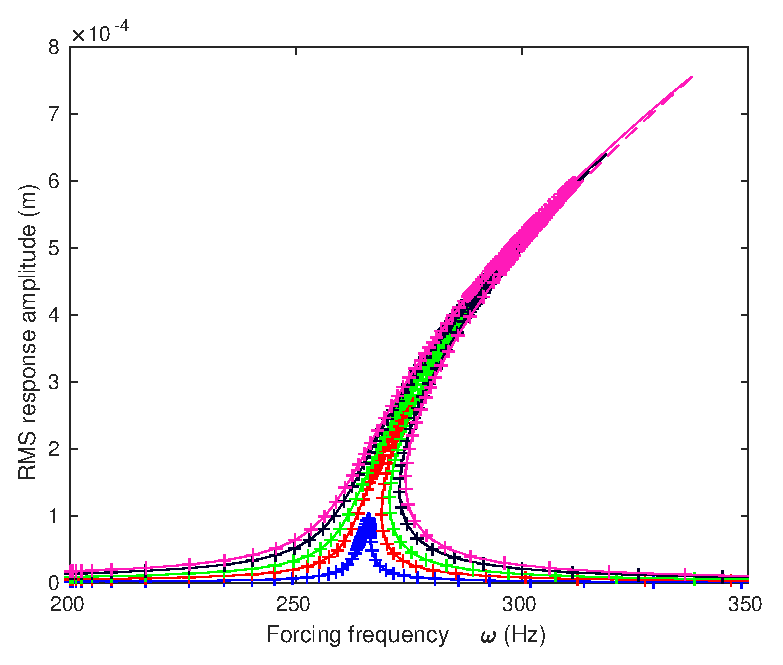
\includegraphics[width=\linewidth]{{../../../benchmark1/fig/pnlssfrf_A0.15_Amp_nx3}.eps}\\
      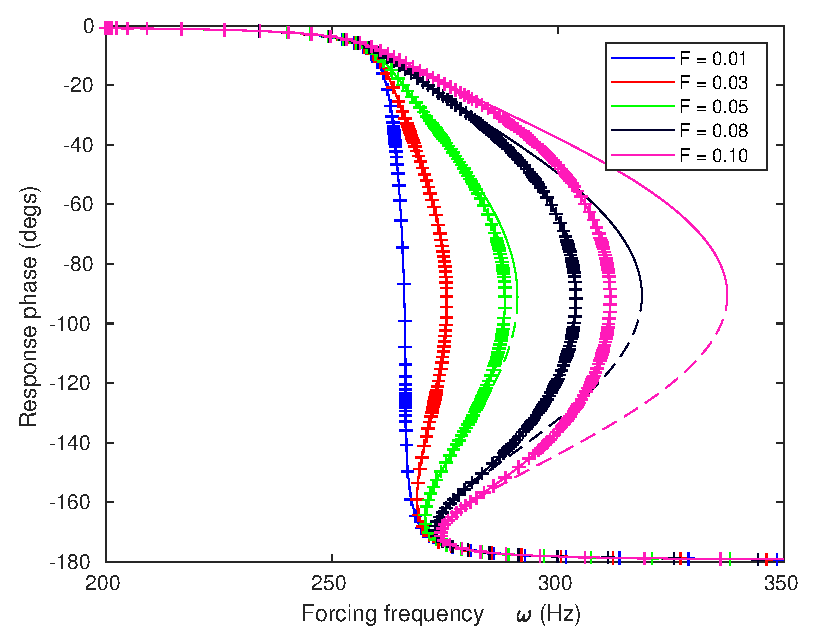
\includegraphics[width=\linewidth]{{../../../benchmark1/fig/pnlssfrf_A0.15_Phase_nx3}.eps}
      \caption{$u_{rms} = 0.15N$}
    \end{subfigure}%
    \begin{subfigure}[t]{0.25\linewidth}
      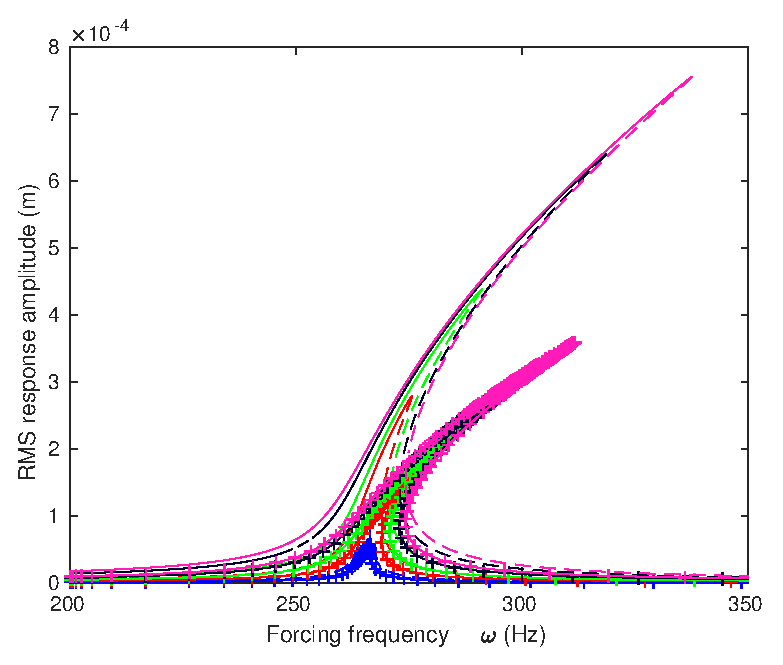
\includegraphics[width=\linewidth]{{../../../benchmark1/fig/pnlssfrf_A0.25_Amp_nx3}.eps}\\
      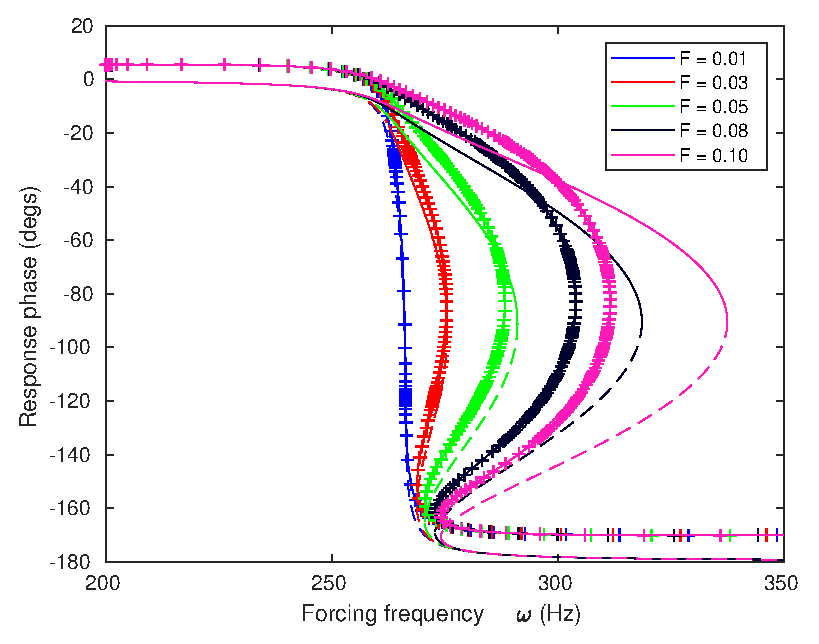
\includegraphics[width=\linewidth]{{../../../benchmark1/fig/pnlssfrf_A0.25_Phase_nx3}.eps}
      \caption{$u_{rms} = 0.25N$ (non-periodic response)}
    \end{subfigure}
    \vspace{-0.75cm}\caption{$n_x=[3]$}
  \end{figure}

  \begin{figure}
    \centering
    \textbf{Sufficiency of non-linear terms}\\
    \begin{subfigure}[t]{0.25\linewidth}
      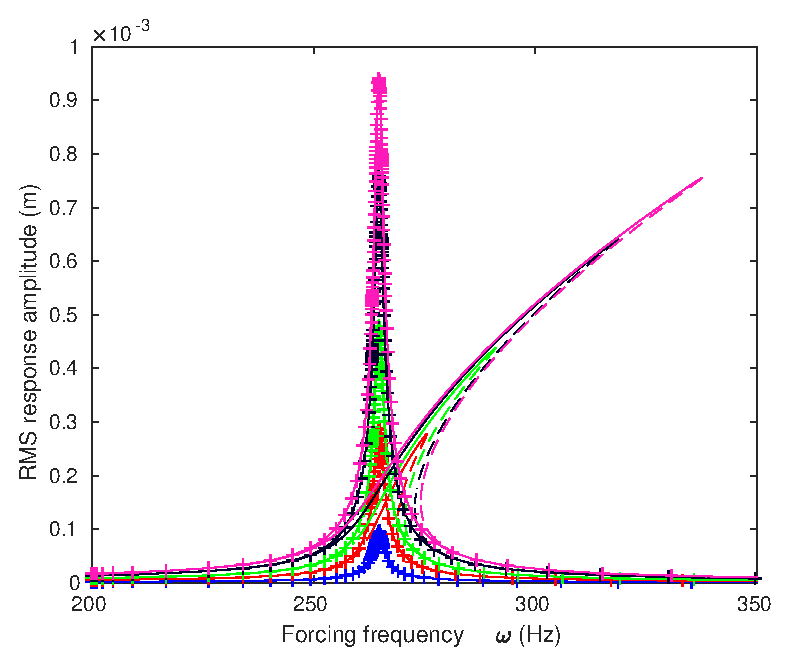
\includegraphics[width=\linewidth]{{../../../benchmark1/fig/pnlssfrf_A0.01_Amp_nx2}.eps}\\
      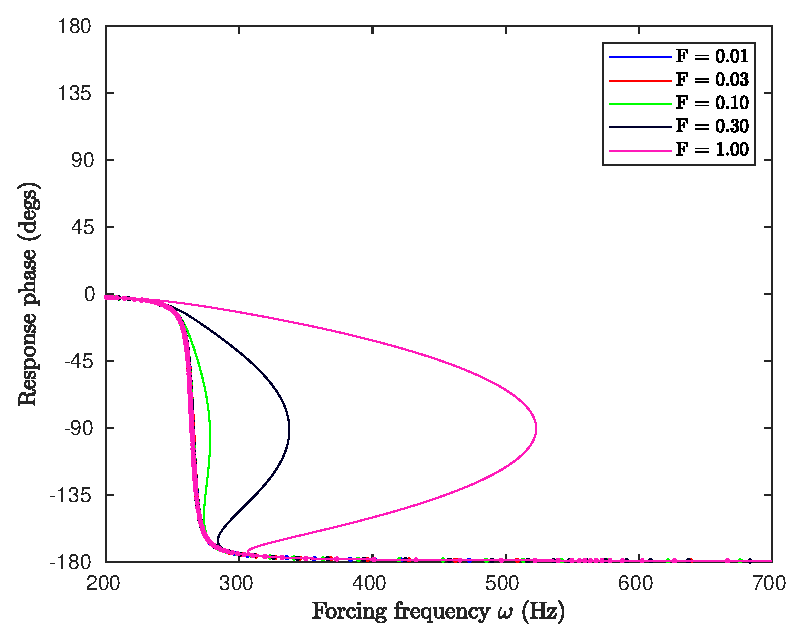
\includegraphics[width=\linewidth]{{../../../benchmark1/fig/pnlssfrf_A0.01_Phase_nx2}.eps}
      \caption{$u_{rms} = 0.01N$}
    \end{subfigure}%
    \begin{subfigure}[t]{0.25\linewidth}
      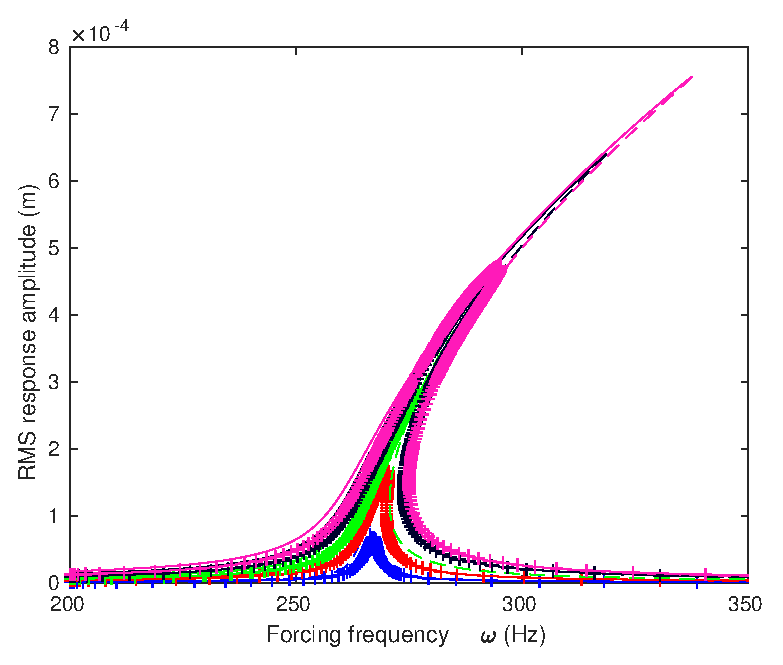
\includegraphics[width=\linewidth]{{../../../benchmark1/fig/pnlssfrf_A0.15_Amp_nx2}.eps}\\
      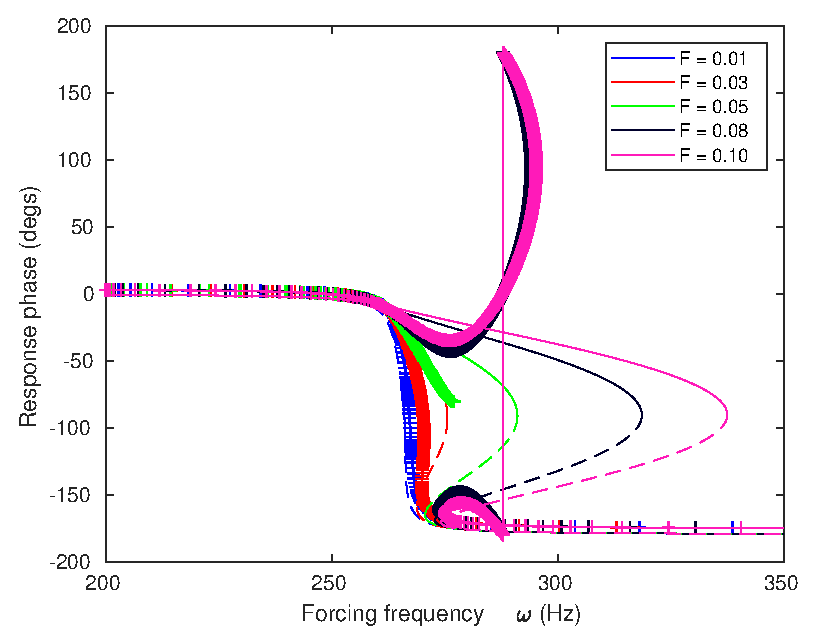
\includegraphics[width=\linewidth]{{../../../benchmark1/fig/pnlssfrf_A0.15_Phase_nx2}.eps}
      \caption{$u_{rms} = 0.15N$}
    \end{subfigure}%
    \begin{subfigure}[t]{0.25\linewidth}
      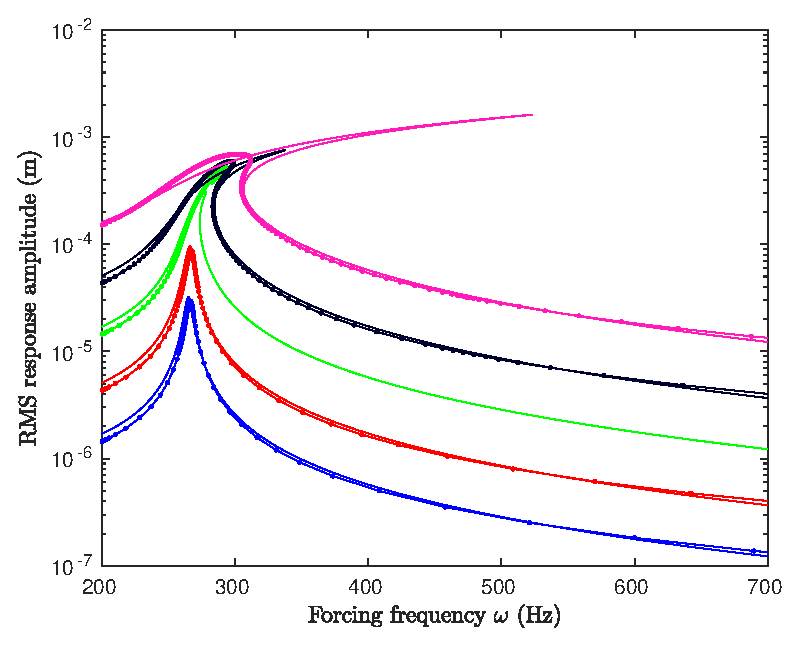
\includegraphics[width=\linewidth]{{../../../benchmark1/fig/pnlssfrf_A0.25_Amp_nx2}.eps}\\
      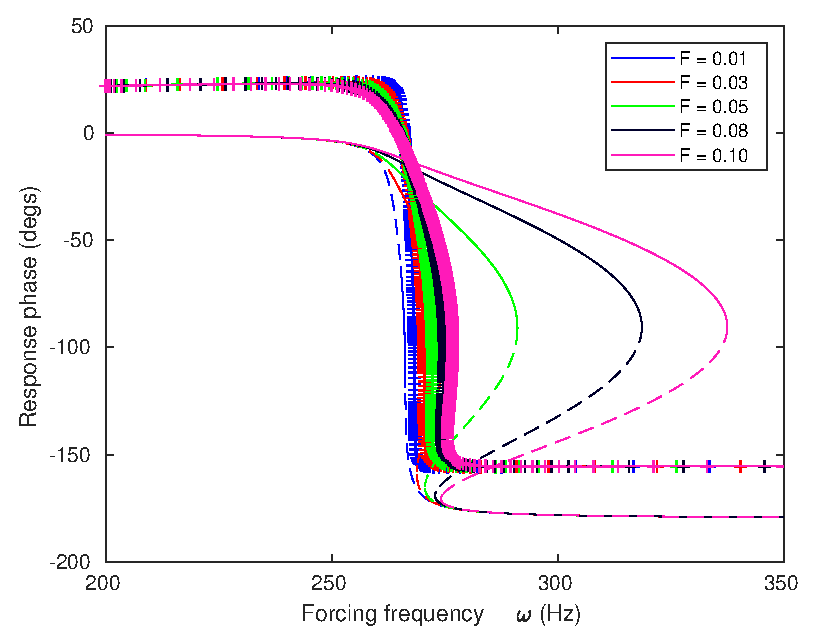
\includegraphics[width=\linewidth]{{../../../benchmark1/fig/pnlssfrf_A0.25_Phase_nx2}.eps}
      \caption{$u_{rms} = 0.25N$ (non-periodic response)}
    \end{subfigure}
    \vspace{-0.75cm}\caption{$n_x=[2]$}
  \end{figure}

  \begin{figure}
    \centering
    \textbf{Sufficiency of non-linear terms}\\
    \begin{subfigure}[t]{0.25\linewidth}
      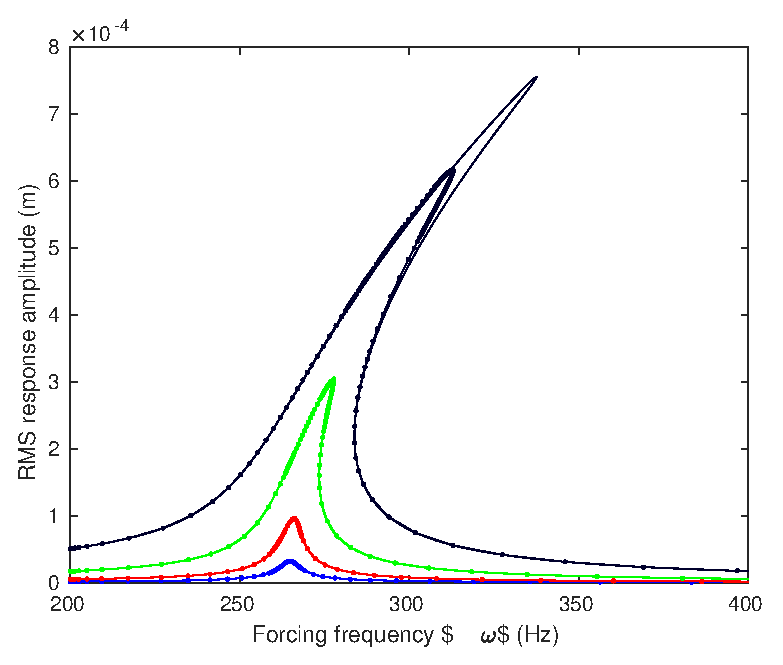
\includegraphics[width=\linewidth]{{../../../benchmark1/fig/pnlssfrf_A0.01_Amp_nx23}.eps}\\
      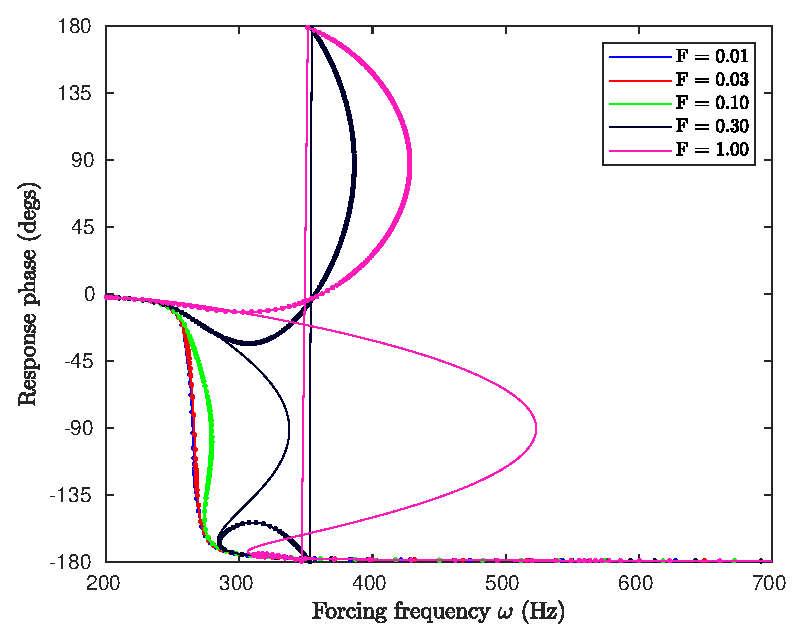
\includegraphics[width=\linewidth]{{../../../benchmark1/fig/pnlssfrf_A0.01_Phase_nx23}.eps}
      \caption{$u_{rms} = 0.01N$}
    \end{subfigure}%
    \begin{subfigure}[t]{0.25\linewidth}
      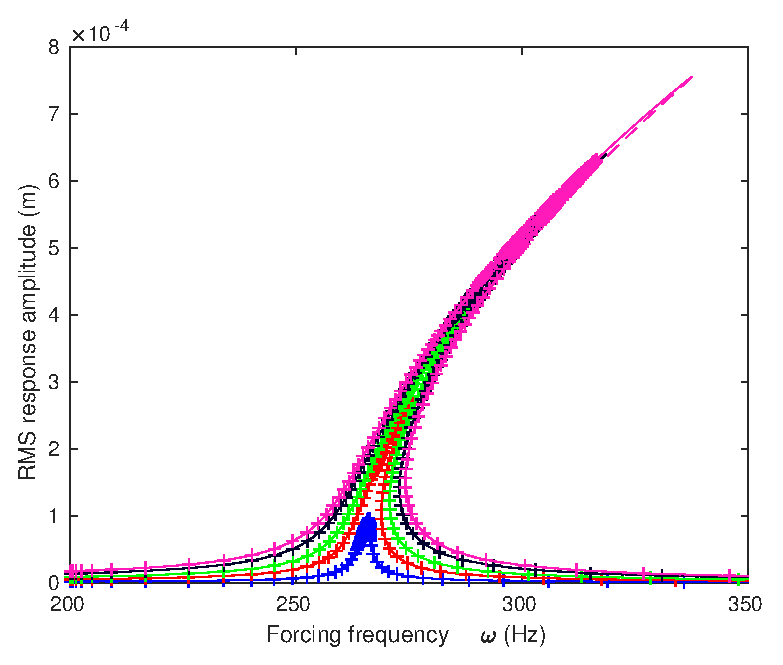
\includegraphics[width=\linewidth]{{../../../benchmark1/fig/pnlssfrf_A0.15_Amp_nx23}.eps}\\
      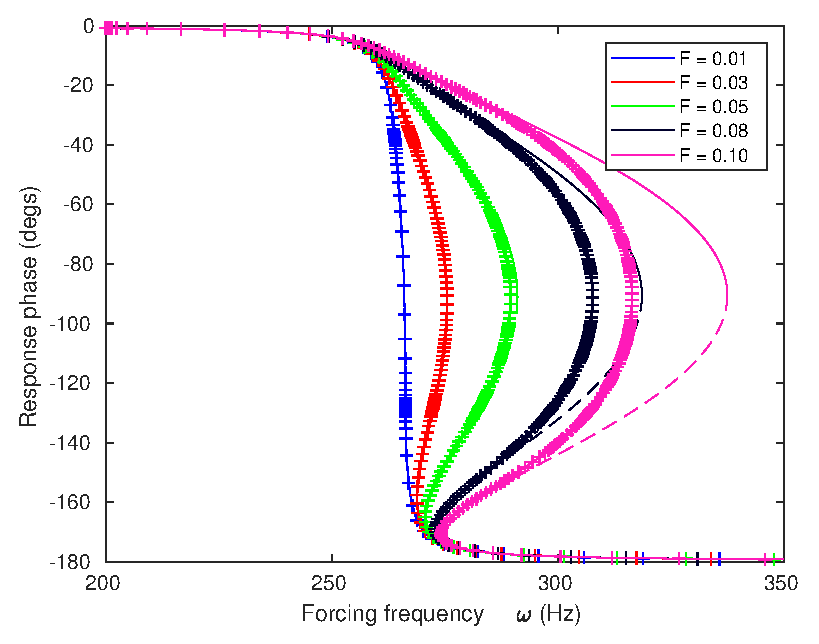
\includegraphics[width=\linewidth]{{../../../benchmark1/fig/pnlssfrf_A0.15_Phase_nx23}.eps}
      \caption{$u_{rms} = 0.15N$}
    \end{subfigure}%
    \begin{subfigure}[t]{0.25\linewidth}
      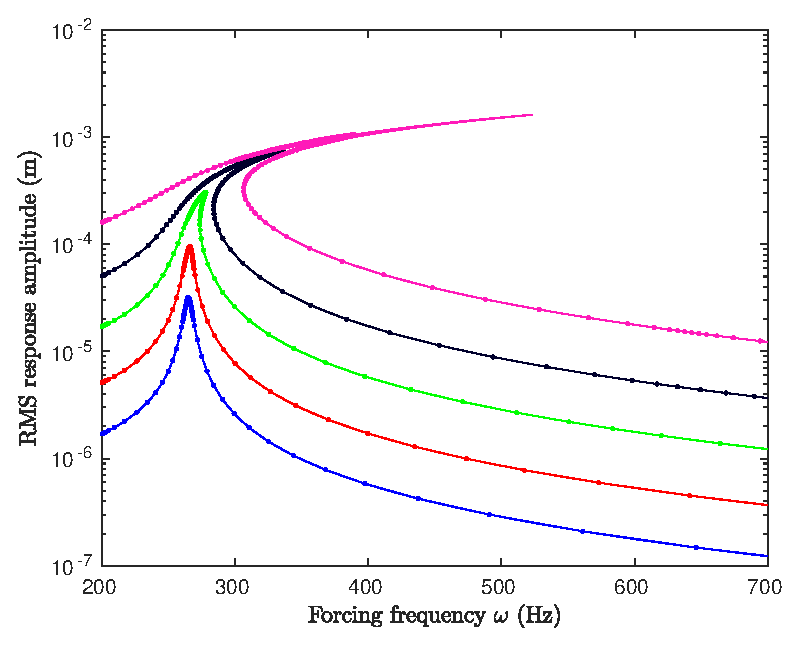
\includegraphics[width=\linewidth]{{../../../benchmark1/fig/pnlssfrf_A0.25_Amp_nx23}.eps}\\
      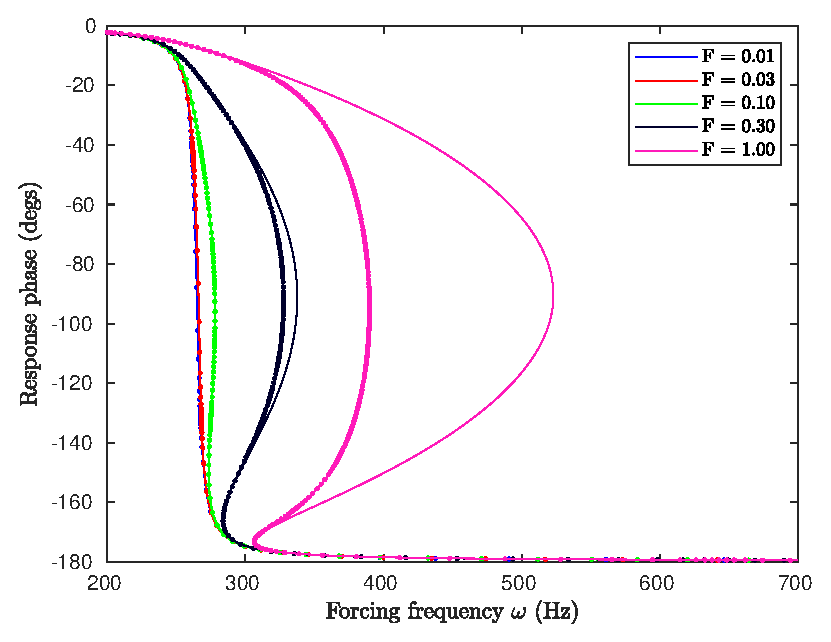
\includegraphics[width=\linewidth]{{../../../benchmark1/fig/pnlssfrf_A0.25_Phase_nx23}.eps}
      \caption{$u_{rms} = 0.25N$ (non-periodic response)}
    \end{subfigure}
    \vspace{-0.75cm}\caption{$n_x=[2, 3]$}
  \end{figure}

  \begin{figure}
    \centering
    \textbf{Sufficiency of non-linear terms}\\
    \begin{subfigure}[t]{0.25\linewidth}
      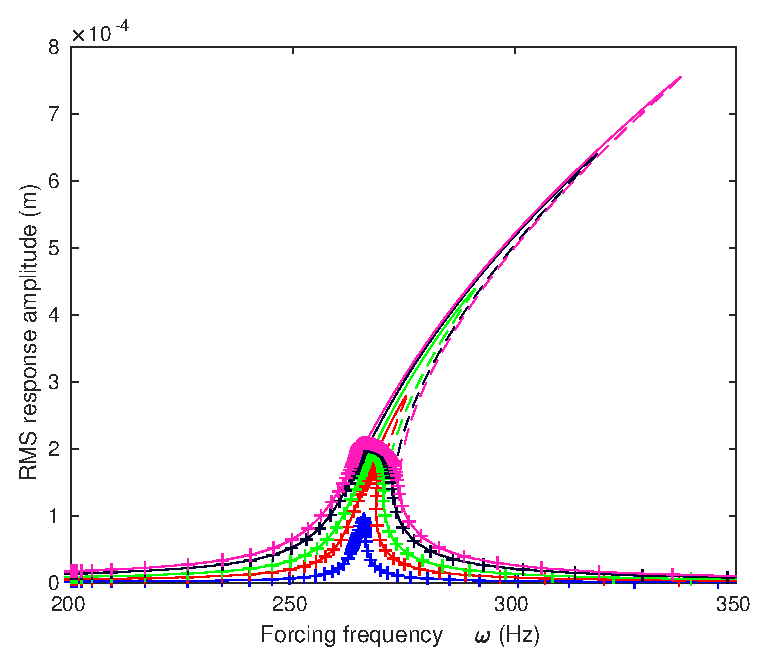
\includegraphics[width=\linewidth]{{../../../benchmark1/fig/pnlssfrf_A0.01_Amp_nx35}.eps}\\
      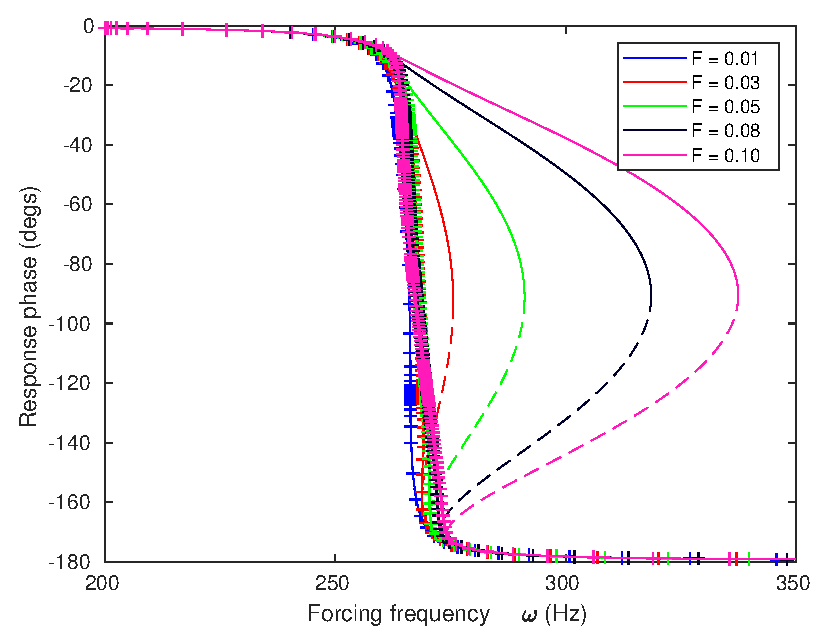
\includegraphics[width=\linewidth]{{../../../benchmark1/fig/pnlssfrf_A0.01_Phase_nx35}.eps}
      \caption{$u_{rms} = 0.01N$}
    \end{subfigure}%
    \begin{subfigure}[t]{0.25\linewidth}
      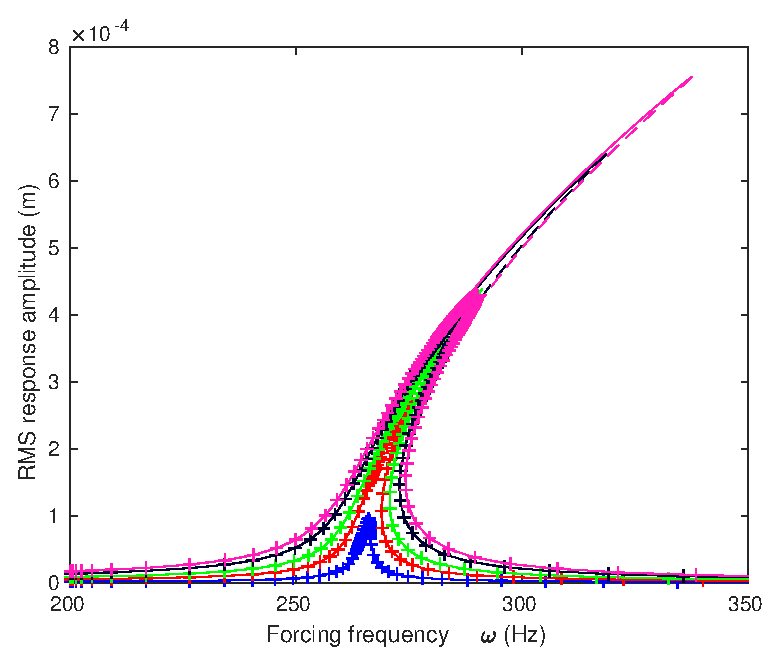
\includegraphics[width=\linewidth]{{../../../benchmark1/fig/pnlssfrf_A0.15_Amp_nx35}.eps}\\
      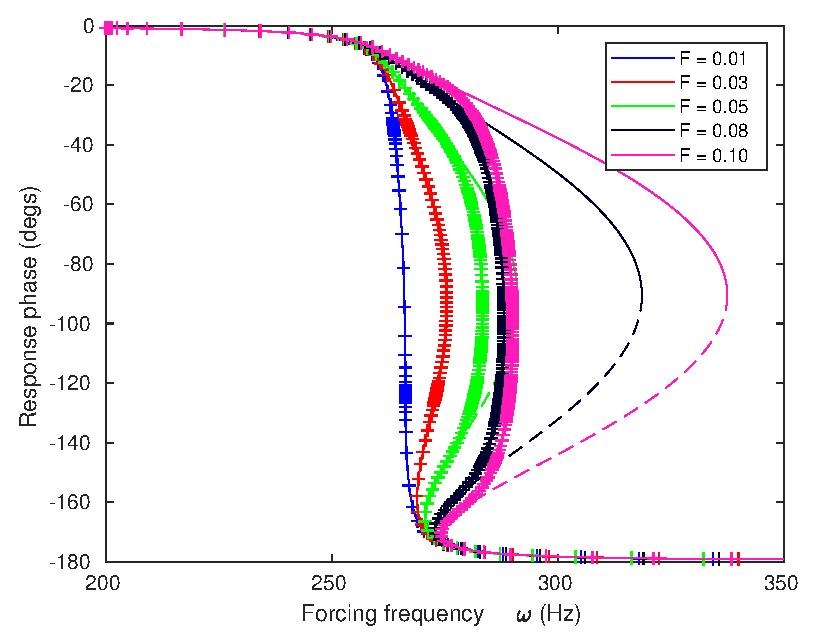
\includegraphics[width=\linewidth]{{../../../benchmark1/fig/pnlssfrf_A0.15_Phase_nx35}.eps}
      \caption{$u_{rms} = 0.15N$}
    \end{subfigure}%
    \begin{subfigure}[t]{0.25\linewidth}
      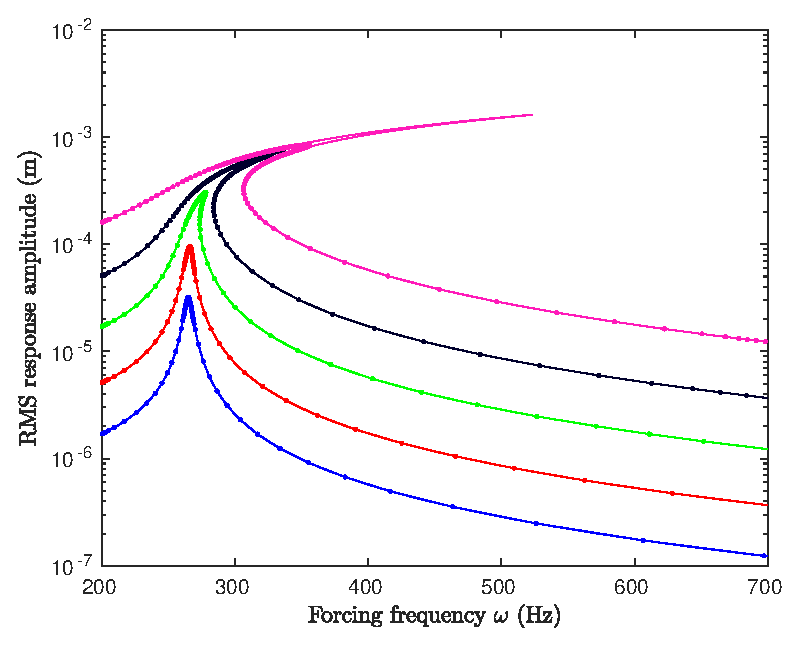
\includegraphics[width=\linewidth]{{../../../benchmark1/fig/pnlssfrf_A0.25_Amp_nx35}.eps}\\
      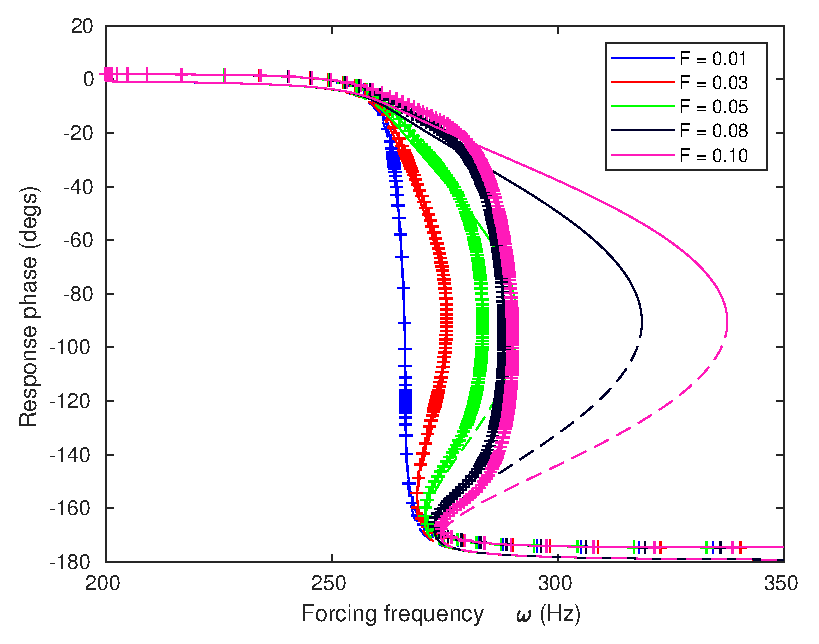
\includegraphics[width=\linewidth]{{../../../benchmark1/fig/pnlssfrf_A0.25_Phase_nx35}.eps}
      \caption{$u_{rms} = 0.25N$ (non-periodic response)}
    \end{subfigure}
    \vspace{-0.75cm}\caption{$n_x=[3, 5]$}
  \end{figure}

  \begin{itemize}
  \item The continuous time model stability estimates are extremely
    unreliable
  \item Possibly something wrong with my implementation - any pointers?
  \end{itemize}
  \begin{figure}
    \centering
    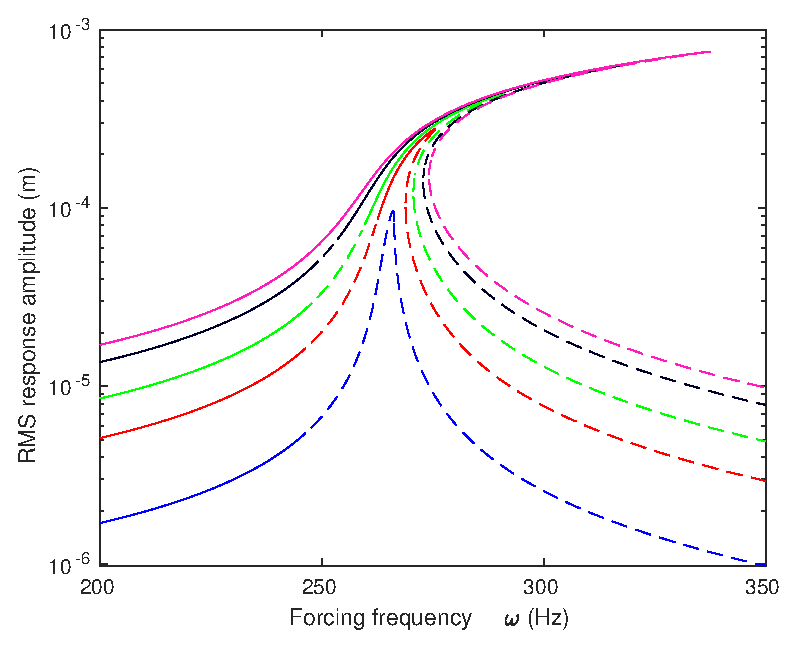
\includegraphics[width=0.4\linewidth]{../../../benchmark1/fig/stabsol_Amp}%
    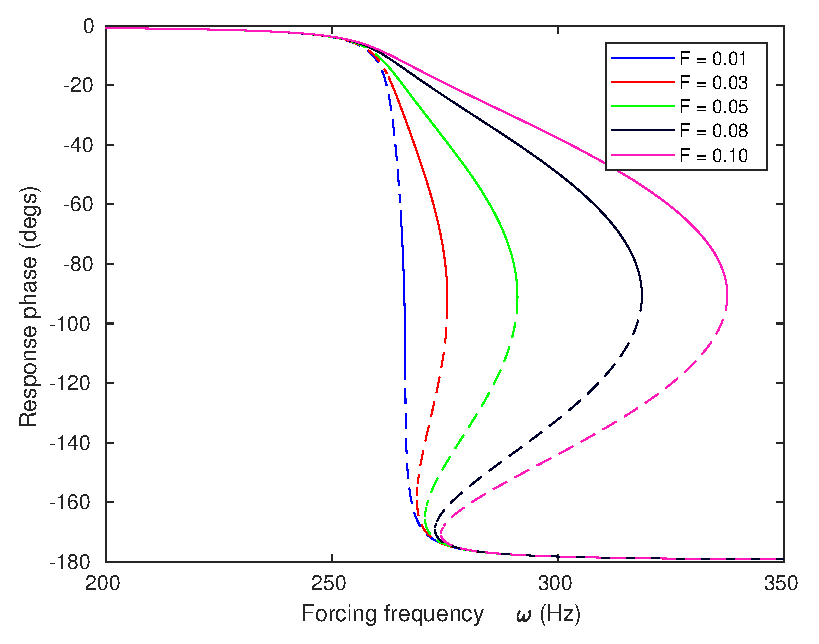
\includegraphics[width=0.4\linewidth]{../../../benchmark1/fig/stabsol_Phase}
    \caption{Frequency response of continuous time model}
  \end{figure}

  \begin{itemize}
  \item The discrete time model stability estimates are even more
    unreliable - shows that no solution is stable!
  \item Something definitely wrong with my implementation - pointers?
  \end{itemize}
  \begin{figure}
    \centering
    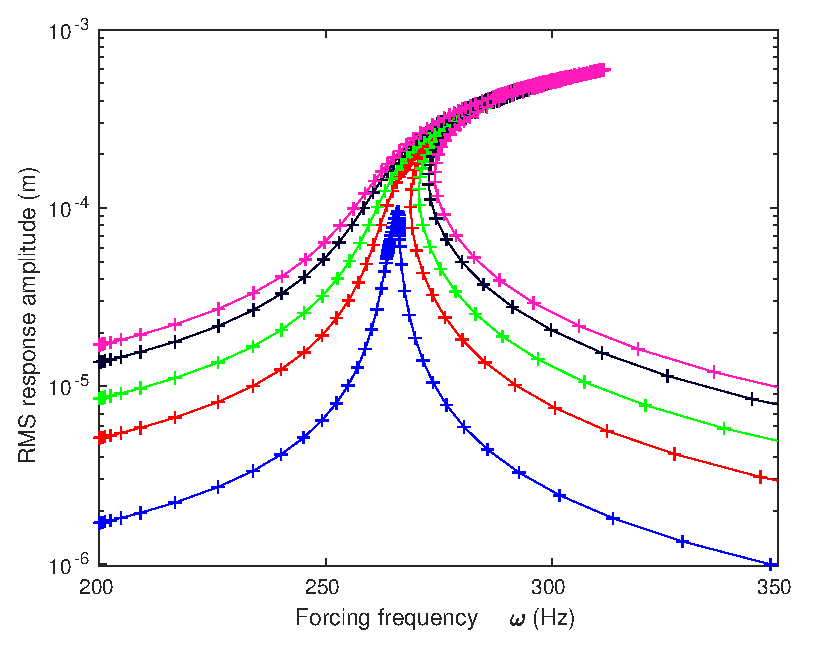
\includegraphics[width=0.4\linewidth]{../../../benchmark1/fig/dtstabsol_Amp}%
    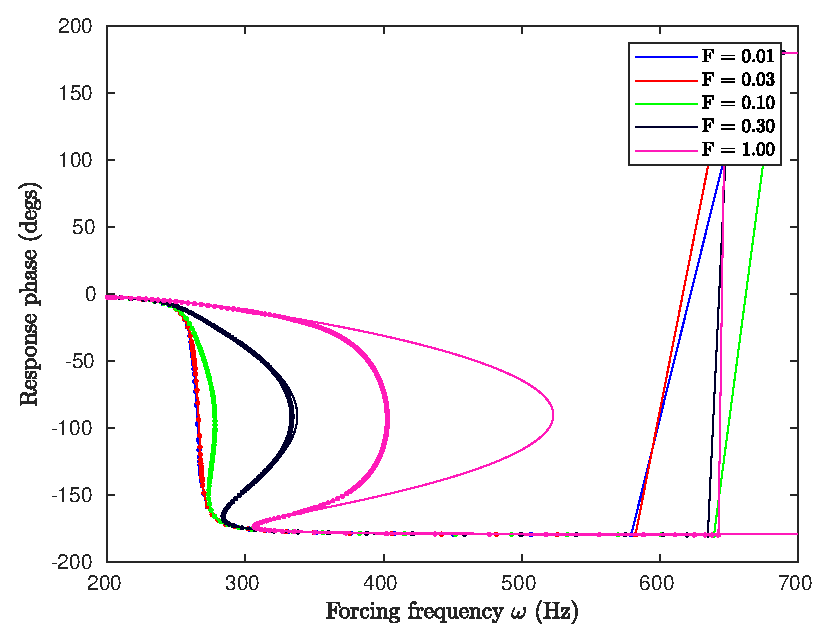
\includegraphics[width=0.4\linewidth]{../../../benchmark1/fig/dtstabsol_Phase}
    \caption{Frequency response of continuous time model}
  \end{figure}  
\end{frame}

\begin{frame}
  \frametitle{Queries}
  \begin{itemize}
  \item Dealing with non-periodic data (periodic input leading to
    non-periodic responses).
    \begin{itemize}
    \item How to go about transient handling? Will it be good to try
      and fit transients too?
    \item Since for non-periodic responses (say, quasi-periodic) the
      starting phase (initial conditions) are very crucial, do we use
      the corresponding routine? We had difficulty in getting this to
      work very well..
    \end{itemize}
  \item Stability exponents in the frequency domain.
    \begin{itemize}
    \item Tips on interpreting hill's coefficients (threshold complex
      angle for instability, etc)
    \item Tips on the exponents for the discrete time models
    \end{itemize}
  \end{itemize}
\end{frame}

\begin{frame}
  \frametitle{Steps forward}
  \begin{enumerate}
  \item Conducting EPMC backbone estimates for the imperfect model (with shaker)
  \item Conducting the PNLSS studies for the MDOF benchmarks
  \item Conducting PNLSS with imperfect model (shaker force as input;
    response as output)
  \item Comparing stability 
  \end{enumerate}
\end{frame}
\end{document}
%%% Local Variables:
%%% mode: latex
%%% TeX-master: t
%%% End:
